\section{Procedure a supporto dei processi}


\subsection{Procedure di progetto}
\label{procedurediprogetto}

Quando non è specificato come modificare il valore di un parametro del ticket bisogna mantenere il valore già presente, o quello di default se il ticket è appena stato creato.

Il parametro ``Tag nel titolo'' corrisponde al testo racchiuso tra parentesi quadre che deve essere posto all'inizio del campo ``titolo'', in aggiunta al titolo esplicito.

\subsubsection{Creazione compito}

\begin{figure}[H]
    \centering
    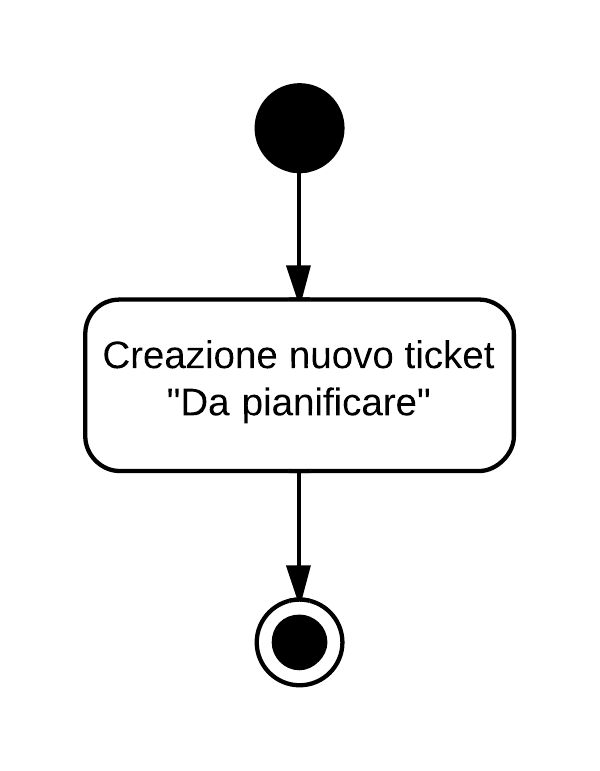
\includegraphics[width=7cm]{uml-processi/Creazione_compito.png}
    \caption{Creazione compito}
\end{figure}

Il Progettista, dopo aver completata la progettazione di dettaglio, deve creare i ticket di codifica con i seguenti parametri:
\begin{itemize}
 \item \textbf{Sezione}:''Da pianificare''
 \item \textbf{Milestone}: la revisione entro la quale il compito dovrà essere terminato.
 \item \textbf{Tag nel titolo}: nessuno.
 \item \textbf{Titolo}: breve descrizione del compito, con il riferimento all'unità di lavoro corrispondente.
 \item \textbf{Dipendenze}: le dipendenze decise nella progettazione.
 \item \textbf{Pianificazione}: nessuna.
 \item \textbf{Assegnato a}: il Responsabile.
\end{itemize}

\subsubsection{Pianificazione compito e verifica}
\label{pianificazione}

\begin{figure}[H]
    \centering
    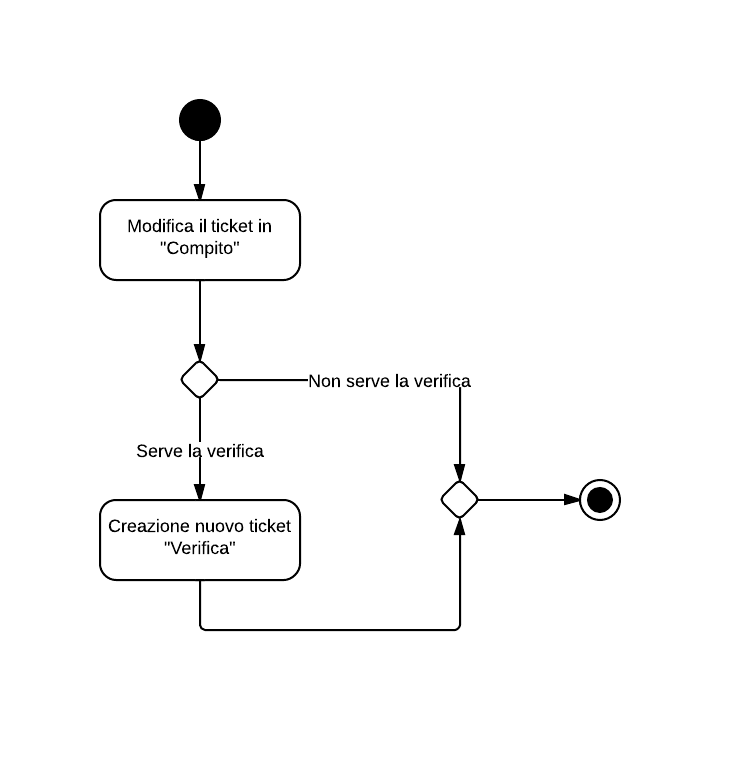
\includegraphics[width=11cm]{uml-processi/Pianificazione_compito_e_verifica.png}
    \caption{Pianificazione compito e verifica}
\end{figure}

Il Responsabile deve pianificare i ticket delle sezioni ``Da pianificare''. Deve inoltre creare e pianificare il corrispondente ticket di verifica se necessario. I ticket del compito e della modifica devono essere assegnati a persone diverse.

Modifica i parametri del compito:
\begin{itemize}
 \item \textbf{Sezione}: ``Compito''.
 \item \textbf{Pianificazione}: a scelta del Responsabile.
 \item \textbf{Assegnato a}: un programmatore, a scelta del Responsabile.
\end{itemize}

Parametri della verifica:
\begin{itemize}
 \item \textbf{Sezione}: ``Verifica''
 \item \textbf{Milestone}: la revisione entro la quale la verifica dovrà essere terminata.
 \item \textbf{Titolo}: breve descrizione della verifica, con un riferimento al compito da verificare.
 \item \textbf{Dipendenze}: il compito di cui bisogna fare la verifica.
 \item \textbf{Pianificazione}: a scelta del Responsabile.
 \item \textbf{Assegnato a}: un verificatore, a scelta del Responsabile.
\end{itemize}

\subsubsection{Esecuzione compito}

\begin{figure}[H]
    \centering
    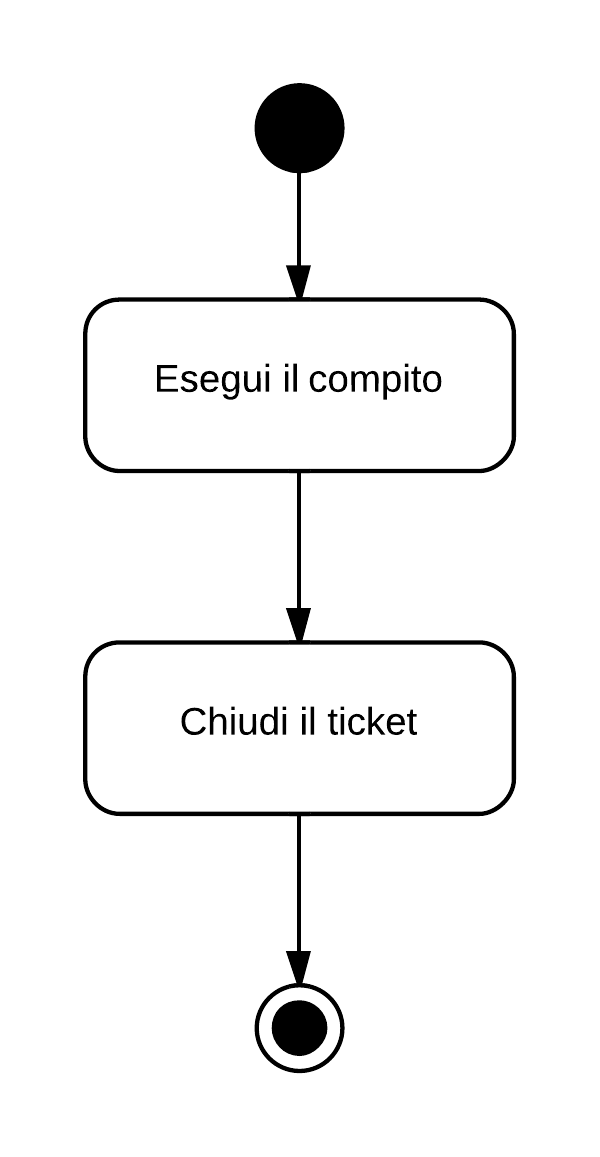
\includegraphics[width=7cm]{uml-processi/Esecuzione_compito.png}
    \caption{Esecuzione compito}
\end{figure}

Non appena il programmatore a cui è assegnato un ticket comincia a lavorare deve impostare una percentuale maggiore di $0\%$. Quando termina il compito deve chiudere il ticket:
\begin{itemize}
 \item \textbf{Stato}: ``Chiuso''.
\end{itemize}
 
\subsubsection{Esecuzione verifica}

\begin{figure}[H]
    \centering
    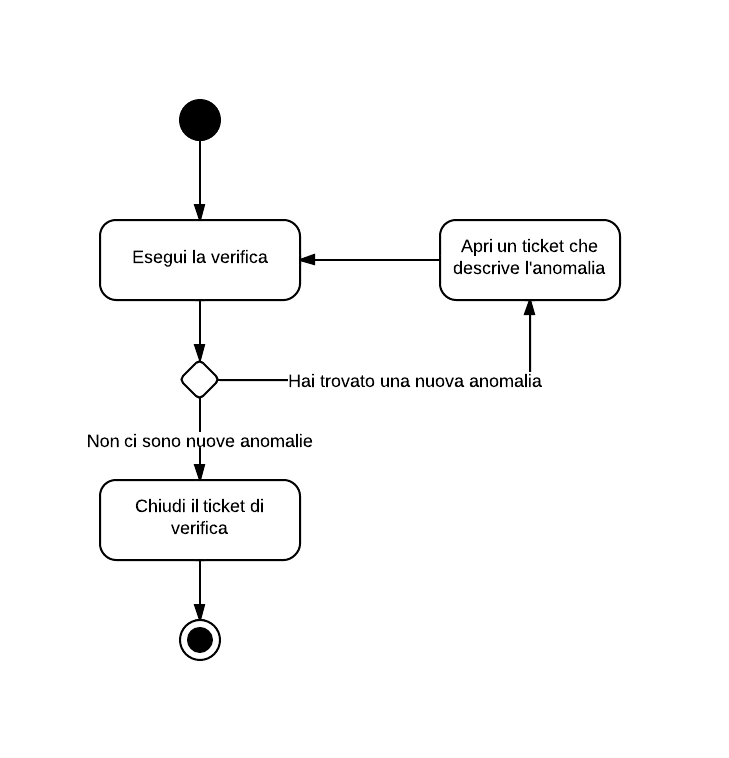
\includegraphics[width=11cm]{uml-processi/Esecuzione_verifica.png}
    \caption{Esecuzione verifica}
\end{figure}

Non appena il verificatore a cui è assegnato un ticket comincia a lavorare deve impostare una percentuale maggiore di $0\%$. Quando termina la verifica deve chiudere il ticket:
\begin{itemize}
 \item \textbf{Stato}: ``Chiuso''.
\end{itemize}

Nel caso in cui il verificatore trovi bug o non conformità significative deve creare un ticket di tipo ``Da valutare'':
\begin{itemize}
 \item \textbf{Sezione}: ``Da valutare''
 \item \textbf{Milestone}: la revisione entro la quale il bug dovrà essere corretto, è opzionale.
 \item \textbf{Tag nel titolo}: un aggettivo tra ``Error'', ``Fault'', ``Failure'', ``Mistake'', come descritto nel \PianoDiQualifica.
 \item \textbf{Titolo}: breve descrizione del bug, con un riferimento al compito nel quale lo si è trovato.
 \item \textbf{Dipendenze}: nessuna.
 \item \textbf{Pianificazione}: nessuna.
 \item \textbf{Assegnato a}: il Responsabile.
\end{itemize}

\subsubsection{Valutazione delle modifiche}

\begin{figure}[H]
    \centering
    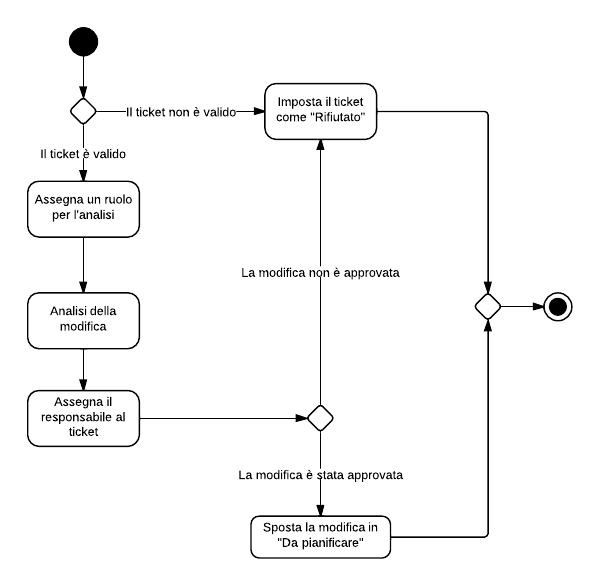
\includegraphics[width=1.2\textwidth]{uml-processi/Valutazione_delle_modifiche.png}
    \caption{Valutazione delle modifiche}
\end{figure}

Il Responsabile deve valutare ogni modifica del tipo ``Da valutare''. Se la formulazione della modifica è corretta allora la assegna ad un ruolo competente:
\begin{itemize}
 \item \textbf{Assegnato a}: un membro del gruppo a scelta del Responsabile
\end{itemize}

Tale ruolo, dopo averla analizzata, deve riassegnarla al Responsabile aggiungendo le informazione prodotte dall'analisi:
\begin{itemize}
 \item \textbf{Assegnato a}: il Responsabile
 \item \textbf{Descrizione}: la descrizione già presente con in aggiunta i risultati dell'analisi.
\end{itemize}

A questo punto, se il Responsabile ritiene che la modifica debba essere eseguita, imposta i seguenti parametri:
\begin{itemize}
 \item \textbf{Sezione}: ``Da pianificare''
 \item \textbf{Milestone}: la revisione entro la quale la modifica dovrà essere fatta.
\end{itemize}
e passa a pianificare il ticket, seguendo la procedura \ref{pianificazione}.

Se il Responsabile non approva o non è ritene valida la modifica deve impostare:
\begin{itemize}
 \item \textbf{Sezione}: ``Rifiutato''.
 \item \textbf{Assegnato a}: nessuno.
 \item \textbf{Stato}: ``Chiuso''.
\end{itemize}

\subsubsection{Richiesta di modifica e segnalazione bug}
\label{segnalazionebug}

\begin{figure}[H]
    \centering
    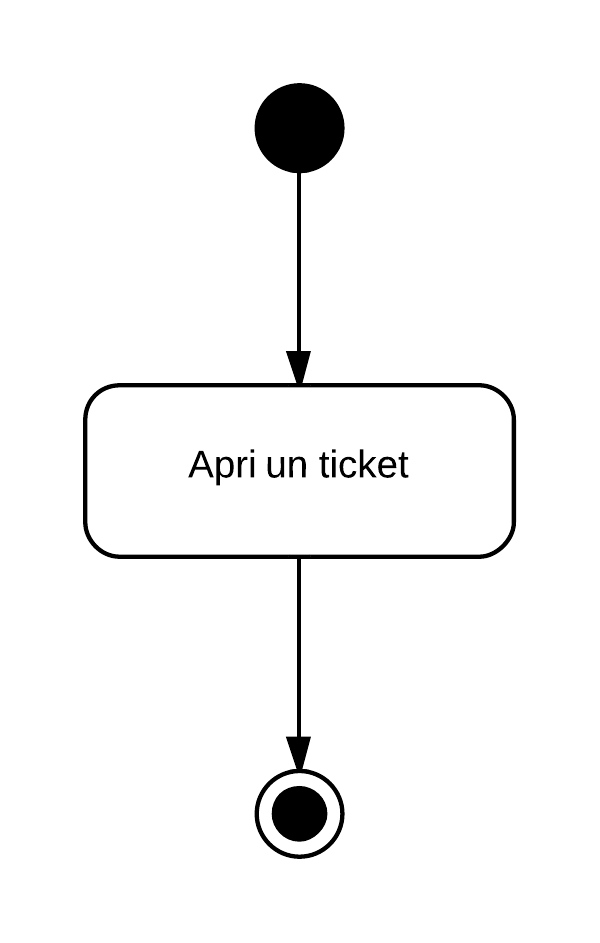
\includegraphics[width=7cm]{uml-processi/Richiesta_di_modifica_e_segnalazione_bug.png}
    \caption{Richiesta di modifica e segnalazione bug}
\end{figure}

Se un membro del gruppo volesse segnalare un bug o richiedere una modifica deve creare un ticket con i seguenti parametri:
\begin{itemize}
 \item \textbf{Sezione}: ``Da valutare''
 \item \textbf{Milestone}: la revisione entro la quale la modifica dovrà essere fatta, è opzionale.
 \item \textbf{Tag nel titolo}: un aggettivo tra ``Error'', ``Fault'', ``Failure'', ``Mistake'', come descritto nel \PianoDiQualifica, oppure ``Modifica'' se è una richiesta di modifica.
 \item \textbf{Titolo}: breve descrizione della modifica.
 \item \textbf{Descrizione}: descrizione completa e auto-sufficiente del bug o della modifica richiesta.
 \item \textbf{Dipendenze}: nessuna.
 \item \textbf{Pianificazione}: nessuna.
 \item \textbf{Assegnato a}: il Responsabile.
\end{itemize}


\subsection{Analisi dei requisiti}

Dal capitolato e dagli incontri con il proponente gli Analisti dovranno estrarre i requisiti del progetto, producendo l'Analisi dei Requisiti.

Tutti i requisiti che si possono evincere dal capitolato o ad un incontro con il proponente vanno specificati nell'Analisi dei Requisiti.

Per agevolare l'analisi dei requisiti viene utilizzata la tecnica dei casi d'uso.

    \subsubsection{Tracciamento requisiti}
     I requisiti vengono tracciati mediante il software \emph{Requisteak} appositamente creato dal gruppo \GroupName{}. Tale strumento è raggiungibile all'indirizzo:
     \begin{center}
         \url{http://steakholders.herokuapp.com}.
     \end{center} 
     Le credenziali di accesso sono le seguenti:
     \begin{itemize}
        \item \textbf{Username}: \texttt{committente@steakholders.com};
        \item \textbf{Password}: \texttt{unipd2013}.
     \end{itemize}
     
\subsubsection{Casi d'Uso}

Ogni caso d'uso dovrà presentare i seguenti campi:
\begin{itemize}
 \item Codice identificativo
 \item Titolo
 \item Diagramma UML
 \item Attori primari
 \item Attori secondari 
 \item Scopo e descrizione
 \item Precondizione
 \item Postcondizione
 \item Flusso principale degli eventi
 \item Scenari alternativi
\end{itemize}

\subsubsection{Codice identificativo}

Ogni caso d'uso è identificato da un codice, che segue il seguente formalismo:
\begin{center}
    \code{UC\{X\} \{Gerarchia\}}
\end{center}

Dove:
\begin{itemize}
 \item \textbf{X} corrisponde all'ambito di riferimento e può assumere i seguenti valori:
    \begin{itemize}
     \item[] \textbf{U} = Ambito \glossario{Utente};
     \item[] \textbf{S} = Ambito \glossario{Sviluppatore}.
    \end{itemize}

     \item \textbf{Gerarchia} identifica la relazione gerarchica che c'è tra i casi d'uso di uno stesso ambito. C'è quindi una struttura gerarchica per ogni ambito dei casi d'uso. La numerazione potrebbe non essere continua nel caso in cui vengano rimossi alcuni degli use case numerati in precedenza.
\end{itemize}

\subsubsection{Requisiti}

Ogni requisito dovrà presentare i seguenti campi:
\begin{itemize}
 \item Codice identificativo
 \item Descrizione
 \item Fonti
\end{itemize}

\subsubsection{Codice identificativo}

Ogni requisito è identificato da un codice, che segue il seguente formalismo:
\begin{center}
    \code{R\{X\}\{Y\}\{Z\} \{Gerarchia\}}
\end{center}

Dove:
\begin{itemize}
 \item \textbf{X} corrisponde al sistema di riferimento e può assumere i seguenti valori:
    \begin{itemize}
     \item[] \textbf{A} = Applicazione \glossario{Maap};
     \item[] \textbf{F} = \glossario{Framework} di \glossario{Maap};
     \item[] \textbf{S} = \glossario{Maas}.
    \end{itemize}

 \item \textbf{Y} corrisponde alla tipologia del requisito e può assumere i seguenti valori:
    \begin{itemize}
     \item[] \textbf{1} = Funzionale;
     \item[] \textbf{2} = Di prestazione;
     \item[] \textbf{3} = Di qualità;
     \item[] \textbf{4} = Vincolo.
    \end{itemize}

 \item \textbf{Z} corrisponde alla priorità del requisito e può assumere i seguenti valori:
    \begin{itemize}
     \item[] \textbf{O} = Obbligatorio
     \item[] \textbf{D} = Desiderabile
     \item[] \textbf{F} = Facoltativo o opzionale
    \end{itemize}

 \item \textbf{Gerarchia} identifica la relazione gerarchica che c'è tra i requisiti di uno stesso tipo. C'è quindi una struttura gerarchica per ogni tipologia di requisito.
\end{itemize}

\subsubsection{UML}

Per i diagrammi deve essere utilizzata il linguaggio \emph{UML versione 2.0}.


\subsection{Progettazione}
%\subsubsection{Specifica Tecnica}
La progettazione deve dimostrabilmente rispettare tutti i requisiti che il gruppo ha concordato con il committente. In particolare i componenti progettati devono essere tracciabili rispetto al requisito che soddisfano.
Di seguito vengono elencate le norme a carico dei \emph{Progettisti}.

    \subsubsection{Diagrammi UML}
    Si dovrà usare il linguaggio \glossario{UML} \emph{versione 2.0} per i seguenti diagrammi:
\begin{itemize}
 \item \textbf{Diagrammi dei package:} dovranno essere presenti sia per l'architettura generale che di dettaglio, sarà fondamentale per definire i moduli all'interno del \glossario{framework} \glossario{Node.js} richiesto dal capitolato;
 \item \textbf{Diagrammi delle classi:} qualora il progetto utilizzasse delle classi, i diagrammi delle classi dovranno essere presenti sia per l'architettura generale che di dettaglio. Nell'ambiente \glossario{Node.js} a prima vista sembra che siano poco utilizzate, a favore dei \glossario{package};
 \item \textbf{Diagrammi di flusso:} qualora la codifica di un'unità del progetto sia particolarmente complessa, dovrà essere presente il relativo diagramma di flusso che il programmatore dovrà seguire;
\end{itemize}

    \subsubsection{Stile di progettazione}
    \begin{itemize}
        \item La progettazione dovrà usare quanto più possibile \glossario{design pattern} globalmente affermati, la loro scelta dovrà essere giustificata;
        \item Suddividere il progetto in \glossario{moduli}, in accordo con lo stile di progettazione dell'ambiente \glossario{Node.js};
        \item Non utilizzare codice sincrono per operazioni di \glossario{I/O};
        \item Limitare quanto più possibile le \glossario{callback} annidate;
    \end{itemize}


    %\paragraph{Test di integrazione}
    %I test di integrazione avvengono mediante la definizione e l'utilizzo di opportuni strumenti di test per verificare che i componenti del sistema funzionino nella maniera prevista.


%\subsubsection{Definizione di Prodotto}
%La \emph{Definizione di Prodotto} è la descrizione dettagliata della progettazione descritta nella \emph{Specifica Tecnica}. Questo documento rappresenta lo stadio avanzato della progettazione e indicherà ogni singolo componente del sistema permettendo ai \emph{Programmatori} di procedere con lo sviluppo. Parallelamente alla progettazione di dettaglio dovranno essere progettati i relativi test di unità che verranno descritti nel \PianoDiQualifica .

%   \paragraph{Definizione di classe}
%   Le classi progettate devono comparire nella \emph{Definizione di Prodotto} che dovrà descriverne l'elenco dei metodi e degli attributi, lo scopo e la funzionalità che rappresenta.
%   completare...
%   
%   % \subsubsection{Formalismo di specifica dei metodi}
%    \subsubsection{Tracciamento classi}
%   
%   \paragraph{Test di unità}
%   I \emph{Progettisti} modellano i test da effettuare sulle unità per le opportune verifiche.



%\subsubsection{Verifica della progettazione architetturale}
%\subsubsection{Verifica della progettazione di dettaglio}
%\subsubsection{Verifica del codice}
%\paragraph{Analisi Statica}
%\paragraph{Analisi Dinamica}
%\subsection{Resoconto bug}
%\subsection{Validazione output}

%\subsection{Codifica}
%   \subsubsection{Codifica e convenzioni}
%       \paragraph{Nomi}
%       \paragraph{Ricorsione}
%   \subsubsection{Documentazione}


\subsection{Codifica}

\subsubsection{Intestazione}

\begin{lstlisting}
/*
* Name: {Nome del file}
* Module: {modulo di appartenenza}
* Location: {/path/della/cartella/}
*
* History:
* Version     Date            Programmer    
* ================================================
* 1.1.3       AAAA-MM-GG      {Nome Cognome      }
* ------------------------------------------------
* ...
* {Description}
* ...
* ================================================
* 1.1.2       AAAA-MM-GG      {Nome Cognome      }
* ------------------------------------------------
* ...
*
*/
\end{lstlisting}

\begin{itemize}
 \item \textbf{Name} è il nome del file, estensione compresa.
 \item \textbf{Module} è il nome del modulo di cui il file fa parte.
 \item \textbf{Location} è il percorso del file, a partire dalla cartella principale del progetto ``/'' fino alla cartella che contiene il file. Deve iniziare e terminare con uno slash ``/".
 \item \textbf{History} è il diario delle modifiche del file. Ogni modifica è composta dai seguenti campi:
 
    \begin{itemize}
     \item \textbf{Version} è la versione del file.
     \item \textbf{Date} è la data della modifica.
     \item \textbf{Programmer} è il nome e cognome dell'autore della modifica. Al massimo può essere lungo 20 caratteri.
     \item \textbf{Description} è la spiegazione delle modifiche fatte e del motivo per cui sono state fatte.    
    \end{itemize}
\end{itemize}

\subsubsection{Formattazione}

La formattazione del codice sorgente deve essere definita in modo rigoroso e consistente, così che tutto il codice del progetto sembri che sia stato scritto da un'unica persona.

Per il codice \emph{Javascript} si è scelto di adottare le linee guida utilizzate dal progetto \emph{jQuery}, sia per l'effettiva facilità di lettura sia per la possibilità di automatizzare la formattazione del codice tramite il programma \emph{JSHint}. La pagina di riferimento è \url{http://contribute.jquery.org/style-guide/js/}.

%\paragraph{Indentazione}
%\subsubsection{Norme di validazione}
%\subsubsection{Rendiconto ore}
%\paragraph{Nomi}
%\paragraph{Disciplina}
%\subsubsection{Protocolli vari}